\documentclass[10pt,a4paper]{article}

\usepackage[colorlinks=true,urlcolor=blue,linkcolor=blue]{hyperref}
\usepackage[utf8]{inputenc}
\usepackage[T1]{fontenc}
\usepackage[french]{babel}
\usepackage{fancyvrb}
\usepackage{tikz}
\usepackage{pgf-umlsd}
\usepgflibrary{arrows}

\usepackage{float}
\usepackage{graphicx}

\title{Cahier des besoins - Reversi}
\author{Guillaume CHUPIN, Benoit FAGET, Alexis PICHON, Julien PILLEUX}

\begin {document}
\maketitle
\newpage
\tableofcontents
\newpage

\section{Introduction}

Notre projet consiste en l'élaboration d'un joueur de Reversi complet développé en suivant certaines règles afin de pouvoir être confronté à d'autre implémentations au cours d'un tournoi prévu qui confrontera notre programme à celui d'une seconde équipe de développement ayant reçu le même sujet.\\

Nous avons eu le choix entre utiliser le langage de programmation C ou le C++, nous avons décidé de prendre le C++. Notre programme appliquera les algorithmes les plus fréquents pour un joueur de Reversi et utilisera au mieux les bitboards. Un bitboard est une structure de donnée qui est très efficace pour encoder un plateau de jeu tel que celui du reversi, un bitboard est un ensemble de bit ou chaque bit correspond a une case du plateau et indique la présence ou l'absence d'une pièce, ainsi on devra utilisé deux bitboard, un pour la présence de pion blanc et un autre pour la présence de pion noir.  L'interface utilisateur sera purement en mode texte dans un bash, on se concentrera plutôt sur le développement d'heuristiques propres au jeu. Le projet sera essentiellement dirigé vers l'utilisation de techniques d'exploration d'arbre classiques telles que Minimax-ab, Negamax, Negascout, MTD(f), Monte-Carlo Tree Search (MCTS), etc. Il nous reste à définir laquelle développer en première, et si nous aurons le temps d'en faire d'autres.

\section{Description et analyse de l'existant}

Le jeu de Reversi consiste en un jeu de pions opposant deux adversaires dont le but est de terminer avec le plus grand nombre de pions à la fin de la partie. La partie se termine lorsque plus aucun mouvement n'est possible pour chacun des deux joueurs. Un joueur ne peut placer un pion que sur une case vide adjacente a un pion adverse et que si le pion ainsi posé permet la capture d'au moins un pion adverse. Pour capturer les pions adversaires, il faut que ceux-ci se retrouve entre un de vos pions déjà présent et celui que vous vous apprêtez à poser sur le plateau. La capture de pions peut s'effectuer dans les huit directions à la fois (voir Fig \ref{fig:aire_de_capture}).
 \begin{figure}[H]    
    \centering
\begin{tikzpicture}

  \node (x) {X};
  \node (r) at (0.8,0) {};
  \node (ru) at (0.63,0.63) {};
  \node (u) at (0,0.75) {};
  \node (lu) at (-0.63, 0.63) {};
  \node (l) at (-0.8, 0) {};
  \node (ld) at (-0.63, -0.63) {};
  \node (d) at (0, -0.75) {};
  \node (rd) at (0.63, -0.63) {};
  
  \draw[->] (x) -- (r);
  \draw[->] (x) -- (ru);
  \draw[->] (x) -- (u);
  \draw[->] (x) -- (lu);
  \draw[->] (x) -- (rd);
  \draw[->] (x) -- (d);
  \draw[->] (x) -- (ld);
  \draw[->] (x) -- (l);
  \end{tikzpicture}
    \caption {Aire de capture d'un pion.\label{fig:aire_de_capture}}
    \end{figure}
\subsection{Stratégies}
%%%%%%%%%%%%%%%%%%%%%%%%%%%%%%%%%%%%%%%A voir si on l'enlève%%%%%%%%%%%%%%%%%%%%%%%%%%%%%%%%%%%%%%%%%%%%%%%%%%%%%%%%%%
Différentes stratégies autour du jeu existent. En effet, certaines positions sont meilleures que d'autres, car offrant moins de possibilités à l'adversaire de la reprendre, si ce n'est aucune. Par exemple, les quatre coins du plateau font parties de ces positions imprenables. De plus, une fois ces positions prises, les positions adjacentes deviennent également imprenables, et ainsi de suite (voir Fig \ref{fig:bord_stable}).

 \begin{figure}[H]    
    \centering
    \begin{BVerbatim}
       1 2 3 4 5 6
     A X _ _ _ _ X
     B _ _ _ _ _ _
     C _ _ _ _ _ _
     D _ _ _ _ _ _
     E _ _ _ _ X X
     F X _ _ _ X X 
    \end{BVerbatim}
    \caption {Les bords stable.\label{fig:bord_stable}}
    \end{figure}

D'autres positions imprenables sont celles qui se retrouvent entre des pions adverses, car ce dernier ne pourra pas non plus les reprendre. Par exemple, dans la Fig \ref{fig:exemple_insertion}, on peut voir que le joueur noir (représenté par un 'X') peut effectuer une insertion en jouant en 'A3', le joueur blanc ne pourra pas reprendre ce pion. Au tour suivant, quelque soit le coup du joueur blanc, le joueur noir pourra jouer en 'A1' et ainsi avoir un des coins si désirés, lui permettant ainsi de gagner en stabilité en possédant maintenant trois pions indétronables.
 \begin{figure}[H]    
    \centering
    \begin{BVerbatim}
       1 2 3 4 5 6
     A _ O _ O _ _
     B _ _ O O _ _
     C _ _ X _ _ _
     D _ _ _ _ _ _
     E _ _ _ _ _ _
     F _ _ _ _ _ _ 
    \end{BVerbatim}
    \caption {Exemple d'insertion.\label{fig:exemple_insertion}}
    \end{figure}
Une autre stratégie reviendrait à diminuer le nombre de coups de l'adversaire tout en augmentant son propre nombre de coups, pour cela on va privilégier les coups rapportant le moins de pions, mais tout en faisant attention à ce que l'adversaire ne puisse pas nous enlever tous nos pions. Réduire le nombre de coups de l'adversaire n'est pas tout, il faut aussi tendre à ne lui laisser la possibilité de ne jouer que des mauvais coups.\\

Comme nous pouvons l'observer à travers les différentes stratégies, nous aurons besoin d'explorer les arbres des coups possibles, mais la complexité d'une telle démarche devient rapidement gigantesque, nous empêchant de parcourir en un temps raisonnable l'arbre en entier. Fort heureusement, nous n'aurons pas besoin de le parcourir en entier, car nous pourrons déterminer que certaines branches de l'arbre ne valent pas le coup d'être explorées.
%%%%%%%%%%%%%%%%%%%%%%%%%%%%%%%%%%%%%%%%%%%%%%%%%%%%%%%%%%%%%%%%%%%%%%%%%%%%%%%%%%%%%%%%%%%%%%%%%%%%%%%%%%%%%%%%%%%%%%%%%%%%%%%%%ùùù
\subsection{Programmes}
%%%%%%%%%%%A Détailler%%%%%%%%%%%%%%%%%
Dans les années 80, le programme qui était le champion à ce jeu se nommait Iago. Il se basait sur les stratégies énoncées précédemment, mais de part la contrainte technique de temps due aux tournois, ils ont dû utiliser certaines astuces. Ainsi, le programme calcule pour chaque coup le temps qu'il peut passer sur celui-ci. Ensuite, durant le temps alloué pour chaque coup, il recherche dans son arbre jusqu'à une profondeur de 7, qu'ils ont jugée comme étant la profondeur donnant le meilleur résultat dans un temps restreint. Pour réduire son temps de réponse, ils ont aussi amélioré les fonctions d'évaluation, mais ils ont surtout réduit le nombre de noeuds que le programme devra examiner.
\newpage
%%%%%%%%%%%%%%%%%%%%%%%%%%%%%%%%%%%%%%%
\section{Besoins fonctionnels}
\label{sec:besoins_fonctionnels}

\subsection {Déroulement d'une partie}
\label{sec:deroulement_partie}

% Diagrammes de séquences
\begin{figure}[H]
  \centering
  \begin{sequencediagram}
    % Instances
    \newthread[blue]{user}{User} %[couleur]{nom 'variable'}{nom affichage}
    \newthread[green]{game}{Reversi} % [distance]
    \tikzstyle{inststyle}+=[bottom color=white, top color=white, rounded corners = 3mm]
    \newinst[4]{board}{Plateau} 

    % Instanciation Plateau
    \begin{messcall}{user}{./reversi}{game} % {source}{affichage}{destination}
      \begin{call}{game}{create\_board()}{board}{Display rules and board} % {source}{affichage}{destination}{retour}
      \end{call}
    \end{messcall}

    % Le joueur joue un coup
    \mess{user}{Play move}{game} % L'utilisateur choisi une case
    \begin{call}{game}{play\_move(String)}{board}{update\_display()} % Le jeu passe la chaîne correspondante au plateau
      \begin{call}{board}{check\_if\_valid()}{board}{valid OR not valid} % Le plateau vérifie la validité du mouvement.
      \end{call}
    \end{call}

    % La machine joue à son tour
    \begin{call}{game}{ia\_play\_move(String)}{board}{update\_display()} % Normalement pas besoin de vérifier (si on code ça bien).
    \end{call}

    % Le joueur décide de quitter
    \mess{user}{Enter q}{game}
    \mess{game}{Ask save}{user}
    \mess{user}{Type y}{game}
    \begin{call}{game}{save\_game()}{board}{}
    \end{call}
    \begin{call}{game}{quit()}{game}{}
    \end{call}
    
  \end{sequencediagram}
  \caption{Diagramme séquentiel de déroulement d'une partie.\label{fig:diagramme_partie}}
\end{figure}

\subsection{Listes des fonctionnalités}
\label{sec:fonctionnalites}

% Début nouvelle partie post TD1
\begin {itemize}
\item  L'entrée de l'utilisateur est insensible à la casse.
\item  L'utilisateur peut choisir un coup à jouer en entrant les coordonnées de la case où il désire jouer, par exemple il peut choisir la case \verb!a2!.
\item  L'utilisateur peut sauvegarder sa partie à tout moment en entrant le caractère 'q'. Le fichier de sortie de la sauvegarde est un fichier \verb!ASCII! contenant l'état actuel du plateau plus le tour du prochain joueur (voir Fig. \ref{fig:exemple_save}).
  \begin{figure}[H]    
    \centering
    \begin{BVerbatim}
      O
      _ _ _ _ _ _
      _ _ _ _ _ _
      _ _ X O _ _
      _ _ O X _ _
      _ _ _ _ _ _
      _ _ _ _ _ _ 
    \end{BVerbatim}
    \caption {Exemple de fichier de sauvegarde.\label{fig:exemple_save}}
    \end{figure}

\item  Le programme doit contenir un mode contest permettant de faire s'affronter deux intelligences artificielles. Ce mode de jeu prend en entrée un fichier de sauvegarde obtenu lorsque l'on quitte le programme.
\item  La taille du plateau de jeu est modifiable grâce grâce à une option de lancement. Lors du lancement -s ou --size suivit d'une valeur entre 1 et 5 ce qui fait varier la taille de la grille de 2 à 10 cases en ne prenant que des valeur paires (Voir Fig. \ref{fig:exemple_taille}). Par défaut, la grille affichée sera de dimension \verb!8x8!.
  \begin{figure}[H]    
    \centering
    \begin{BVerbatim}
        1 2 3 4 
      A _ _ _ _
      B _ _ _ _
      C _ _ _ _
      D _ _ _ _
      
    \end{BVerbatim}
    \caption {Exemple de grille générée avec l'option \textsc{-s2}.\label{fig:exemple_taille}}
  \end{figure}
\item  Il est possible de décider quel rôle donner à l'ia lors du lancement du programme.
  \begin{description}
  \item [-w, --white] Pour indiquer que l'ia jouera les pions blancs.
  \item [-b, --black] Pour indiquer que l'ia jouera les pions noirs.
  \item [-a, --all] Pour indiquer que l'ia jouera les deux camps.
  \end{description}
\item  La version du programme sera affichable avec l'option de lancement -V. 
\item  Le mode verbose de la partie sera activable au lancement du programme avec l'option -v. % Fleury a dit qu'il s'en battait les couilles du mode verbose hein.
\item  Une aide est disponible pour l'utilisateur grâce à l'option -h ou --help. Elle liste l'ensemble des options du programme ainsi que leur description.
\end{itemize}
% Fin nouvelle partie post TD1.

\newpage
\section{Besoins non fonctionnels}

\begin{itemize} 
\item Rapidité d'exécution : chaque coup doit être exécuté en moins d'une seconde.
\item Portabilité : le programme doit pouvoir s'exécuter sur toute machine de type Linux..
\item Confiance : les règles doivent être respectées et les fichiers de sauvegarde doivent suivre le format et la forme attendue (voir \ref{fig:exemple_save}).
\end{itemize}

\begin{figure}[H]
\centering
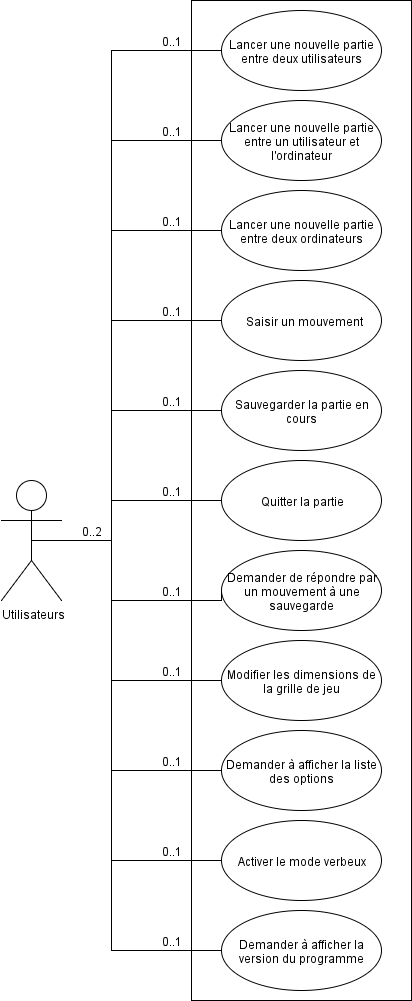
\includegraphics[scale=0.5]{images/use_case.png}
\label{use_case}
\caption{Diagramme de cas d'utilisation}
\end{figure}

\section{Diagramme de Gantt}

\section{Bibliographie}

\end{document}
